\chapter{二维监督下人和物体空间关系的先验学习}\label{chap:super2d}
学习人和物体之间空间关系的先验对于人和物体交互关系的单目重建或者对于理解人如何和周围的物体发生交互关系至关重要,然而,获取人和物体空间关系的先验具有一定挑战性。前置章节(章节\ref{chap:stackflow}和章节\ref{chap:stackflow_plus})所提出的算法依赖于从准确的三维标注数据中学习这些先验知识,由于三维标签数据难以获取并且从实验室采集的数据和自然场景下的数据存在较大的域差异,这些方法难以泛化到多样性丰富的自然场景中,为了克服这些缺陷,本章提出了一种使用二维信息监督的方式从大规模的二维数据学习人-物三维空间关系先验的方法。

该方法将从图片中提取的人和物体的二维关键点按照摄像机姿态反投影到三维空间中得到2.5D的中间表示,利用多视角下关键点的几何一致性来对图片进行聚类,得到每一个人和物体交互类型在各个视角下人-物二维关键点的分布,最后使用基于归一化流的模型从这些数据中学习该分布,以提取人和物体的交互先验。在单目重建优化过程中,通过使用该归一化流模型约束人和物体投影到不同视角下的人和物体关键点来调节人和物体之间的在三维空间中的相对空间位置关系。为了产生更加精细的重建结果,在优化过程中引入接触面损失,从二维图片中统计出人和物体之间在图片中的遮挡区域,综合各个视角下的遮挡区域得到人和物体近似的接触区域,使用该近似的接触区域来拉近人和物体网格模型表面的顶点。为了训练该归一化流模型,从网络上扒取了大量数据并构建了自然场景下的人-物交互数据集,对数据集中图片进行了人-物关键点的标注,该数据集用于训练和测试算法在自然场景中的性能。

为验证该算法的有效性,在室内采集的BEHAVE数据集和自然场景下构建的WildHOI数据集中进行实验。在BEHAVE数据集上,
%使用数据集中提供的摄像机参数和图片中的人-物关键点训练网络,在重建中使用多视角的二维先验来约束重建结果,
将本文所提出的方法和依赖于三维监督的方法进行比较,结果表明该方法在没有直接使用三维标注的情况下,仅仅使用从多视角人和物体二维关键点的排布中学习到的先验来约束人和物体之间的相对空间关系,达到了和使用三维监督的方法相媲美的重建精度。同时,在WildHOI数据集上进一步测试了算法在自然场景中的性能,结果表明在没有使用任何人为构建的先验或利用任何三维的人-物关系标注的前提下,算法有效地重构出自然、合理的人-物空间关系。

\section{多视角二维先验}
\subsection{问题表述}
单视角人和物体联合重建的任务目标在于从给定的图片$\mathbf{I}$中重建出人和物体的三维信息$\mathbf{X}_{\text{3D}}$,为了避免单视角重建自身存在自遮挡或人-物相互遮挡而导致点估计产生的歧义性,一般采用概率化的刻画方式,即从输入图片$\mathbf{I}$中预测出人和物体三维信息的概率密度分布$p(\mathbf{X}_{\text{3D}}|\mathbf{I})$。基于学习的方法需要从海量的数据中建立图片和人-物三维空间关系的对应关系,而由于三维数据标注获取的代价昂贵,很难大规模成批量的采集数据,因而依赖于三维信息监督的方法受限于其学习数据的分布,很难泛化到自然场景中。自然场景中人和物体交互的信息大都以二维图像或视频的形式呈现,互联网上庞大的二维图片数据比三维形式的交互数据更容易搜集和获取,这些二维图片在不同场景和视角下拍摄,自身构成一个天然的多视角拍摄系统。对于同一种交互类型$\mathbf{X}_{\text{3D}}$,在海量的数据中总存在从不同视角下拍摄下的图片,三维信息$\mathbf{X}_{\text{3D}}$在不同视角$\{\rho_1, \rho_2, \dots\}$下经摄像机捕捉系统投影到二维图像平面得到$\{\Pi_{\rho_1}(\mathbf{X}_{\text{3D}}), \Pi_{\rho_2}(\mathbf{X}_{\text{3D}}), \dots\}$,这些二维信息间接地反映了人和物体在三维空间中位置关系。

\begin{figure}[!htbp]
	\centering
	\includegraphics[width=0.8\linewidth]{Img/intro_2d_prior}
	\bicaption{\centering{学习先验示例图}}{\centering{This figure depicts the prior learned from unlimited 2D images in the wild.}}
	\label{fig:intro-2d-prior}
\end{figure}

基于此观察,本章提出从大规模的、更容易获取的二维数据中学习人-物三维空间关系先验的方法,如图\ref{fig:intro-2d-prior}所示,该方法综合各个视角下的二维信息的概率分布来推测出原三维信息的概率密度分布,学习得到的先验被应用于自然场景中的人-物重建。定义图片$\mathbf{I}$所对应三维信息$\mathbf{X}_{\text{3D}}$的评估函数
\begin{equation}\label{eq:score_function}
	S(\mathbf{X}_{\text{3D}}|\mathbf{I}) = \int_{\rho \sim \varrho} p(\Pi_{\rho}(\mathbf{X}_{\text{3D}}), \rho|\mathbf{I}) \text{d}{\rho},
\end{equation}
式中,$\rho$为摄像机位姿,$\Pi_{\rho}$为在位姿$\rho$下的摄像机透视投影函数,$\varrho$为摄像机位姿的概率分布。在实际应用中,$p(\mathbf{X}_{\text{3D}}|\mathbf{I})$是难以获取的,而分布$p(\Pi_\rho(\mathbf{X}_{\text{3D}}), \rho| \mathbf{I})$是容易从大规模图像数据中获取的,通过式(\ref{eq:score_function})将三维信息$\mathbf{X}_{\text{3D}}$投影到各个摄像机图像平面得到$\Pi_\rho(\mathbf{X}_{\text{3D}})$,综合各个视角下的二维信息的分布$p(\Pi_\rho(\mathbf{X}_{\text{3D}}), \rho| \mathbf{I})$来得到原三维信息密度分布$p(\mathbf{X}_{\text{3D}}|\mathbf{I})$的近似评估$S(\mathbf{X}_{\text{3D}}|\mathbf{I})$。

\subsection{人-物关键点}
存在几种方式来刻画人和物体的在图片中几何信息,诸如蒙版、稀疏关键点、密集坐标点等,为了在计算的高效性和几何信息的完整性之间达成平衡,选择稀疏的关键点来刻画人和物体。对于人体,使用SMPL模型中的22个身体关节作为人的关键点,在SMPL模型局部坐标系中,人体关键点的坐标$\mathbf{X}_{\text{3D}}^{\text{SMPL}}\in\mathbb{R}^{22 \times 3}$由人体形状参数$\mathbf{\beta}$和人体姿态参数$\mathbf{\theta}$决定,其计算方式如下,
\begin{equation}\label{eq:smpl-joints}
	\mathbf{X}_{\text{3D}}^{\text{SMPL}} = \mathbf{J}\mathcal{B}(\mathbf{\beta}, \mathbf{\theta}),
\end{equation}
式中,$\mathcal{B}$为蒙皮函数,它将$\mathbf{\beta},\mathbf{\theta}$映射到SMPL网格模型的6890个顶点坐标,$\mathbf{J}\in\mathbb{R}^{22 \times 6890}$为节点权重矩阵,它衡量各个顶点对关节点的贡献程度。对于物体,关键点从物体的网格模型表面的顶点人为地根据物体的几何特征选取,选取的关键点在物体局部坐标系下的位置为$\hat{\mathbf{X}}_{\text{3D}}^{\text{object}} \in \mathbb{R}^{t\times 3}$,$t$为物体关键点的个数,$t$随着物体几何结构的复杂度而在各个物体中取值不同,在SMPL模型局部坐标系下,物体关键点的三维坐标为
\begin{equation}\label{eq:object-kps}
	\mathbf{X}_{\text{3D}}^{\text{object}} = s\hat{\mathbf{X}}_{\text{3D}}^{\text{object}} \mathbf{R}^{\rm{T}} + \mathbf{t},
\end{equation}
式中,$s$为物体的尺度标量,$\mathbf{R},\mathbf{t}$为物体在SMPL模型坐标系下的位姿。人体坐标点和物体坐标相连接得到对人和物体三维信息的表示$\mathbf{X}_{\text{3D}} = \left(\begin{matrix} \mathbf{X}_{\text{3D}}^{\text{SMPL}} \\ \mathbf{X}_{\text{3D}}^{\text{object}} \end{matrix} \right) \in \mathbb{R}^{n\times3}$,$n$为人和物体坐标的个数总和,在基于关键点的表示下,人和物体的参数由信息高度压缩的表示$\{\mathbf{\beta}, \mathbf{\theta}, \mathbf{R}, \mathbf{t}, s\}$转换成形象化的稀疏表达$\mathbf{X}_{\text{3D}}$。

\subsection{三维关键点和二维关键点之间的关系}
在透视摄像机模型下,人-物三维坐标点$\mathbf{X}_{\text{3D}}$其中任何一点$\mathbf{x}_{\text{3D}}\in\mathbf{X}_{\text{3D}}$被投影到图片平面得到该点在图片上的二维坐标$(u,v)$,两者之间的投影关系由下式决定
\begin{equation}\label{eq:projection}
	\lambda \left( \begin{array}{c} u \\ v \\ f \end{array} \right) = \mathbf{R}_{\text{SMPL}} \mathbf{x}_{\text{3D}} + \mathbf{t}_{\text{SMPL}},
\end{equation}
式中,$f$是摄像机的焦距,$\mathbf{R}_{\text{SMPL}}$和$\mathbf{t}_{\text{SMPL}}$是SMPL模型在摄像机坐标系下的位姿,$\lambda$是深度标量。记$\mathbf{x}_{\text{2D}} = (u, v, f)^{\mathrm{T}}, \mathbf{R}_{\text{cam}} = \mathbf{R}_{\text{SMPL}}^{-1}, \mathbf{t}_{\text{cam}}=- \mathbf{R}_{\text{SMPL}}^{-1}\mathbf{t}_{\text{SMPL}}$,重新整理上式并对等式两边归一化得到
\begin{equation}\label{eq:relation_2D_3D}
	\frac{\mathbf{R}_{\text{cam}} \mathbf{x}_{\text{2D}}}{\| \mathbf{R}_{\text{cam}} \mathbf{x}_{\text{2D}}\|} = \frac{\mathbf{x}_{\text{3D}} - \mathbf{t}_{\text{cam}}}{\| \mathbf{x}_{\text{3D}} - \mathbf{t}_{\text{cam}}\|},
\end{equation}
式(\ref{eq:relation_2D_3D})建立起三维空间中关键点$\mathbf{x}_{\text{3D}}$和图片坐标$(u, v)$之间的关系,即给定图片中的观测点$(u, v)$和摄像机的位姿$\{\mathbf{R}_{\text{cam}}, \mathbf{t}_{\text{cam}}\}$,该观测点所对应的三维空间中的点$\mathbf{x}_{\text{3D}}$在以$\mathbf{t}_{\text{cam}}$为起点,以$\mathbf{d}=\frac{\mathbf{R}_{\text{cam}} \mathbf{x}_{\text{2D}}}{\| \mathbf{R}_{\text{cam}} \mathbf{x}_{\text{2D}}\|}$为方向的射线上。按照式(\ref{eq:relation_2D_3D})对人-物关键点中的每一个点计算其方向向量并和$\mathbf{t}_{\text{cam}}$相连得到中间表示
\begin{equation}\label{eq:inter_representation}
	\mathbf{X}_{\text{2.5D}} = \left( \mathbf{d}_1^{\mathrm{T}}, \mathbf{d}_2^{\mathrm{T}}, \dots, \mathbf{d}_n^{\mathrm{T}}, \mathbf{t}_{\text{cam}}^{\rm{T}} \right)^{\mathrm{T}}\in\mathbb{R}^{(n+1)\times 3}.
\end{equation}
在给定摄像机位姿$\{\mathbf{R}_{\text{cam}}, \mathbf{t}_{\text{cam}}\}$的前提下,三维坐标点$\mathbf{X}_{\text{3D}}$和二维坐标点$\mathbf{X}_{\text{2D}}$都可以通过式(\ref{eq:relation_2D_3D})得到中间表示$\mathbf{X}_{\text{2.5D}}$,在实践中,$\mathbf{X}_{\text{3D}}$是难以获取的,但$\mathbf{X}_{\text{2.5D}}$是容易通过式(\ref{eq:relation_2D_3D})中$\mathbf{X}_\text{2D}$从海量图片中搜集的,本章所提出的方法直接从数据中学习$\mathbf{X}_{\text{2.5D}}$的概率密度分布,进而通过式(\ref{eq:relation_2D_3D})来约束$\mathbf{X}_{\text{3D}}$。

\begin{figure}[t]
	\centering
	\includegraphics[width=\linewidth]{Img/pipeline_2d}
	\bicaption{\centering{基于二维先验的人-物重建算法流程图。}}{\centering{The main pipeline of human-object reconstruction method that incorporates with the prior learned from 2D images.}}
	\label{fig:pipeline_2d}
\end{figure}

\section{基于归一化流的先验学习}

如图\ref{fig:pipeline_2d}所示,本章所提出的方法利用归一化流模型从大量自然场景的图片中学习每个图片平面中二维人-物关键点的分布。该归一化流以输入图片$\mathbf{I}$为条件,将来自高斯分布的噪声$\mathbf{z}$转换成2.5D关键点的中间表示$\mathbf{X}_{\text{2.5D}}$,该中间表示结合了视角姿态$\rho$和二维人-物关键点排布$\Pi_\rho(\mathbf{X}_{\text{3D}})$。为了训练该归一化流模型,收集大量来自互联网的图片,并根据每个视角中二维人-物关键点的几何一致性对这些图片进行聚类,使用聚类的结果最优化最大似然来训练该归一化流模型。

\subsection{网络结构}
由于$\mathbf{X}_{\text{3D}}$获取的代价比较昂贵,通过式(\ref{eq:score_function})将其转换到各个视角下$\Pi_{\rho}(\mathbf{X}_{\text{3D}})$的分布,将$\Pi_\rho(\mathbf{X}_{\text{3D}})$和$\rho$通过式(\ref{eq:relation_2D_3D})的等式左边和式(\ref{eq:inter_representation})合并为一个整体得到$\mathbf{X}_{\text{2.5D}}$,使用$p(\mathbf{X}_{\text{2.5D}}|\mathbf{I})$来替代$p(\Pi_\rho(\mathbf{X}_{\text{3D}}), \rho|\mathbf{I})$,使用归一化流来对$p(\mathbf{X}_{\text{2.5D}}|\mathbf{I})$建模。给定图片$\mathbf{I}$作为输入,使用卷积网络提取图片的视觉特征$\mathbf{f}$,归一化流模型以视觉特征$\mathbf{f}$为条件将输入$\mathbf{X}_{\text{2.5D}}$映射到高斯分布中的样本点$\mathbf{z}$,即
\begin{equation}
	\mathbf{z} = \mathcal{F}(\mathbf{X}_{\text{2.5D}};\mathbf{f}),
\end{equation}
归一化流$\mathcal{F}$的结构参照\citet{Glow},由归一化层(actnorm layer)、可逆线性层(invertible $1\times1$ convolusion layer)和解耦层(affine coupling layer)堆叠形成。$\mathbf{X}_{\text{2.5D}}$的概率密度由下式计算
\begin{equation}
	\log p(\mathbf{X}_{\text{2.5D}}|\mathbf{I}) = \log q(\mathbf{z}) - \log \left| \det \frac{\partial \mathcal{F}}{\partial \mathbf{X}_{\text{2.5D}}} \right|^{-1}.
\end{equation}

\subsection{训练}
训练该归一化流模型的目标函数为最小化$\mathbf{X}_{\text{2.5D}}$分布的负对数似然,即
\begin{equation}\label{eq:train-loss}
	\mathcal{L}_{\text{train}} = \mathbb{E}_{\rho \sim \varrho}[- \log p(\Pi_\rho(\mathbf{X}_{\text{3D}}), \rho|\mathbf{I})],
\end{equation}
然而摄像机位姿的分布$\varrho$和每个视角下$\Pi_\rho(\mathbf{X}_{\text{3D}})$的分布是未知的。在从互联网收集的二维图片数据集$\mathcal{D} = \{\mathbf{I}_1, \mathbf{I}_2, \dots\}$中,每张图像自然地存在一个视角$\rho$和一个二维投影$\Pi_\rho(\mathbf{X}_{\text{3D}})$,这显然不足以训练归一化流模型。为了获取每张图片其它视角下相应的二维投影,使用最近邻算法\citep{Dong2011EfficientKN}对图像进行聚类,定义两张图片之间的距离为
\begin{equation}\label{eq:knn_distance}
	d(\mathbf{I}, \mathbf{I}') = \frac{1}{n}\sum_{i=1}^n (\mathbf{d}_i \times \mathbf{d}_i') \cdot (\mathbf{t}_{\text{cam}} - \mathbf{t}_{\text{cam}}'),
\end{equation}
式中$\mathbf{X}_{\text{2.5D}} = \left( \mathbf{d}_1^{\rm{T}}, \mathbf{d}_2^{\rm{T}}, \dots, \mathbf{d}_n^{\rm{T}}, \mathbf{t}_{\text{cam}}^{\rm{T}} \right)^{\rm{T}}$是图片$\mathbf{I}$的中间表示,它通过式(\ref{eq:relation_2D_3D})的等式左边和式(\ref{eq:inter_representation})从图片$\mathbf{I}$的摄像机位姿$\rho$和图片平面上的人-物关键点$\Pi_\rho(\mathbf{X}_{\text{3D}})$计算得出。类似地,${\mathbf{X}_{\text{2.5D}}}' = \left( {\mathbf{d}_1^{\rm{T}}}', {\mathbf{d}_2^{\rm{T}}}', \dots, {\mathbf{d}_n^{\rm{T}}}', {\mathbf{t}_{\text{cam}}^{\rm{T}}}' \right)^{\rm{T}}$是图片$\mathbf{I}'$的中间表征。式(\ref{eq:knn_distance})计算以$\mathbf{t}_{\text{cam}}$为起点、以$\mathbf{d}$为方向的射线和以$\mathbf{t}_{\text{cam}}'$为起点、以$\mathbf{d}'$为方向的射线之间的距离,$d(\mathbf{I}, \mathbf{I}')$的值越小,这些射线越有可能在三维空间中相交,这说明图片$\mathbf{I}$和图片$\mathbf{I}'$包含相同的空间交互类型。这个聚类过程是不需要人为干预的,它输出每张图片$\mathbf{I}$前$k$个邻居所构成的簇
\begin{equation}
	\mathcal{G}_{\mathbf{I}} = \{(\Pi_{\rho_1}(\mathbf{X}_{\text{3D}}), \rho_1, d_1), \dots, (\Pi_{\rho_k}(\mathbf{X}_{\text{3D}}), \rho_k, d_k)\},
\end{equation}
式中$d_i$是图片$\mathbf{I}$和聚簇$\mathcal{G}_{\mathbf{I}}$中第$i$张图片之间的距离。那些与图片$\mathbf{I}$之间的距离大于一定阈值的图片在训练$p(\Pi_\rho(\mathbf{X}_{\text{3D}}), \rho | \mathbf{I})$时被忽略。该最近邻聚类算法具体见算法\ref{alg:knn},该算法遍历数据集中所有存在相同邻居的两张图片$p$和$q$,计算两张图片之间在三维空间的几何距离并更新最近邻集合$\mathcal{G}_p$。算法中相似度SIMILARITY计算方式向量之间的$\ell$-2范数。在训练归一化流的过程中,从聚类$\mathcal{G}_{\mathbf{I}}$中随机选出一批次的数据来最小化目标函数(\ref{eq:train-loss})。

\begin{algorithm}[!htbp]
	\small
	\caption{基于K最近邻的多视角人-物关键点聚类算法}\label{alg:knn}
	\renewcommand{\algorithmicrequire}{\textbf{输入:}}
	\renewcommand{\algorithmicensure}{\textbf{输出:}}
	\begin{algorithmic}[1]
		\Require 数据集每张图片的摄像机位姿和人-物关键点所构成的集合$\mathcal{D}$,迭代次数$n$,最近邻个数$k$,相似度阈值$s$。
		\Ensure 每张图片的聚类结果所构成集合$\{\mathcal{G}_1, \mathcal{G}_2, \dots, \mathcal{G}_m\}$
		\State 随机初始化每张图片的最近邻$\{\mathcal{G}_1, \mathcal{G}_2, \dots, \mathcal{G}_m\}$
		\For {$p \gets 1$ \textbf{to} $m$}
		\State $\mathcal{G}_p' \gets \{ i | p \in \mathcal{G}_i \}$
		\EndFor 
		\State $\text{iter} \gets 1$
		\For {$\text{iter} \gets 1$ \textbf{to} $n$}
		\For {$t \gets 1$ \textbf{to} $m$}
		\For {$p \in \mathcal{G}_t \cup \mathcal{G}_t'$, $q \in \mathcal{G}_t \cup \mathcal{G}_t'$}
		\State $\mathcal{C}_p \gets \{(\Pi_{\rho_i}(\mathbf{X}_{\text{3D}}), \rho_i)|i\in\mathcal{G}_p\}$
		\State $d_{\text{max}} \gets $ $\max_{i \in \mathcal{G}_p} \text{DISTANCE}(\mathcal{C}_p, (\Pi_{\rho_i}(\mathbf{X}_{\text{3D}}), \rho_i))$
		\State $i_{\text{max}} \gets {\arg\max}_{i \in \mathcal{G}_p} \text{DISTANCE}(\mathcal{C}_p, (\Pi_{\rho_i}(\mathbf{X}_{\text{3D}}), \rho_i))$
		\State $d \gets \text{DISTANCE}(\mathcal{C}_p, (\Pi_{\rho_q}(\mathbf{X}_{\text{3D}}), \rho_q))$
		\State $s_{\text{max}} \gets \max_{i\in \mathcal{G}_p} \text{SIMILARITY} ((\Pi_{\rho_i}, \rho_i), (\Pi_{\rho_q}, \rho_q))$
		\If {$d < d_{\text{max}}$ and $s_{\text{max}} < s$}
		\State 将$i_{\text{max}}$从$\mathcal{G}_p$中删除,将$p$从$\mathcal{G}_{i_{\text{max}}}'$中删除
		\State $\mathcal{G}_p \gets \mathcal{G}_p \cup \{q \}, \mathcal{G}_q' \gets \mathcal{G}_q' \cup\{p\}$
		\EndIf 
		\EndFor
		\EndFor
		\EndFor
		\State \Return 每张图片的最近邻$\{\mathcal{G}_1, \mathcal{G}_2, \dots, \mathcal{G}_m\}$		
		%\State
		\Procedure{distance}{$\mathcal{C}$, ($\Pi_\rho(\mathbf{X}_{\text{3D}}), \rho$)}
		\State $x \gets 0$
		\For {$(\Pi_{\rho'} (\mathbf{X}_{\text{3D}}), \rho') \in \mathcal{C}$}
		\State 按照式(\ref{eq:relation_2D_3D})和式(\ref{eq:inter_representation})将 $(\Pi_{\rho'} (\mathbf{X}_{\text{3D}}), \rho')$和$(\Pi_{\rho} (\mathbf{X}_{\text{3D}}), \rho)$分别转换成$\mathbf{X}_{\text{2.5D}}'$和$\mathbf{X}_{\text{2.5D}}$
		\State $x \gets x + d(\mathbf{X}_{\text{2.5D}}, \mathbf{X}_{\text{2.5D}}')$
		\EndFor
		\State $k \gets $ $\mathcal{C}$的元素个数
		\State $x \gets x / k$
		\State \Return $x$
		\EndProcedure
	\end{algorithmic}
\end{algorithm}

\clearpage

\section{带有二维先验的人-物重建算法}
考虑在给定物体形状模板的前提下,从单视角图片中重建人体和物体的任务,在该任务中,人体由SMPL中的形状参数$\mathbf{\beta}$和姿态参数$\mathbf{\theta}$参数化表示,物体由形状模板的旋转矩阵$\mathbf{R}$,平移向量$\mathbf{t}$和尺度标量$s$表示。和大多数方法类似,本章采用了预测-优化两阶段的算法框架从给定的图片$\mathbf{I}$中恢复出参数$\{\mathbf{\beta}, \mathbf{\theta}, \mathbf{R}, \mathbf{t}, s\}$。在第一阶段中使用预先训练好的模型来预测并初始化物体和人体的位姿,之后使用迭代式的优化算法来微调人和物体的位姿。

\paragraph{初始化}
首先使用目前最先进的方法SMPLer-X\citep{NEURIPS2023_2614947a}来预测SMPL的形状参数$\mathbf{\beta}$、姿态参数$\mathbf{\theta}$和SMPL的全局位姿$\{\mathbf{R}_{\text{SMPL}}, \mathbf{t}_{\text{SMPL}}\}$。使用预先训练好的模型CDPN\citep{Li_2019_ICCV}来获取物体的6D位姿$\{\mathbf{R}, \mathbf{t}\}$。物体的尺寸$s$按照物体在现实世界中的大小设置,除此之外使用ViTPose\citep{NEURIPS2022_fbb10d31}来提取图片人体的关键点并使用预训练的CDPN\citep{Li_2019_ICCV}来提取图片中物体的2D-3D对应点坐标。

\paragraph{先验损失}
从大规模二维图片学习的先验可以被灵活的应用到后优化过程中来微调人体的形状$\mathbf{\beta}$和位姿$\mathbf{\theta}$以及物体的6D位姿$\{\mathbf{R}, \mathbf{t}\}$和尺寸$s$。给定输入图片$\mathbf{I}$,使用归一化流模型学习得到的分布$p(\Pi_\rho(\mathbf{X}_{\text{3D}}), \rho | \mathbf{I})$来初始化每个虚拟摄像机的位置$\{\hat{\mathbf{t}}_{\text{cam}}^{(1)}, \dots, \hat{\mathbf{t}}_{\text{cam}}^{(m)}\}$。人和物体的三维关键点$\mathbf{X}_{\text{3D}}$由式(\ref{eq:smpl-joints})和式\ref{eq:object-kps})从$\{\mathbf{\beta}, \mathbf{\theta}, \mathbf{R}, \mathbf{t}, s\}$计算得出,接着这些三维关键点被投影在各个各个虚拟摄像机平面得到中间表示$\{ \hat{\mathbf{X}}_{\text{2.5D}}^{(1)}, \dots,  \hat{\mathbf{X}}_{\text{2.5D}}^{(m)}\}$,这个投影过程对应于式(\ref{eq:relation_2D_3D})的等式右边和式(\ref{eq:inter_representation})。多视角的人-物关键点损失被定义为
\begin{equation}
	\mathcal{L}_{\text{prior}} = - \sum_{i=1}^m \log p(\hat{\mathbf{X}}_{\text{2.5D}}^{(i)}|\mathbf{I}).
\end{equation}
摄像机的位姿$\{\hat{\mathbf{t}}_{\text{cam}}^{(1)}, \dots, \hat{\mathbf{t}}_{\text{cam}}^{(m)}\}$被作为可优化参数和参数$\{\mathbf{\beta}, \mathbf{\theta}, \mathbf{R}, \mathbf{t}, s\}$在后优化过程中一同优化。

\begin{figure}[!htbp]
	\centering
	\includegraphics{Img/acquire_occlusion_maps}
	\bicaption{\centering{人体和物体的平均遮挡图。}}{\centering{The mean occlusion maps of the SMPL and the objects.}}
	\label{fig:acquire_occlusion_maps}
\end{figure}

\paragraph{接触面损失}
除了对人和物体的三维关键点计算损失外,还引入接触面损失来重建出更加细粒度的交互。但接触面对于自然场景中的图片难以被获取。人和物体在三维空间接触会导致人和物体在二维平面的重叠,同样,相反地,接触面可以使用多视角的遮挡图来近似获取。基于这样的想法,使用平均化的遮挡图来近似替代人和物体之间的接触面。记人体模型表面的遮挡图为一个二值矩阵$\mathbf{c}_{\text{h}}\in\mathbb{R}^{6890}$,该矩阵中的元素设置为1代表该点反投影到图片中位于人和物体之间的遮挡区域,而值为0的点表示没有被遮挡。物体遮挡图$\mathbf{c}_{\text{o}}$的定义与$\mathbf{c}_{\text{h}}$类似。为了获得每幅图像的遮挡图,如图\ref{fig:acquire_occlusion_maps}所示,首先把SMPL网格模型和物体网格模型重投影到图像平面上,以获得图像的遮挡蒙版。落入遮挡区域的点被视为被遮挡。根据人的蒙版来决定是正面表面被遮挡还是背面表面被遮挡。这里把靠近图像平面的表面称为正面表面,而远离图像平面的表面称为背面表面。如果SMPL网格正面表面上的顶点的对应投影2D点满足以下条件,则将其视为被遮挡:(1)它落入图像平面的遮挡区域,(2)在其位置的人物蒙版为0。如果SMPL网格背面表面上的顶点的对应投影2D点满足以下条件,则将其视为被遮挡:(1)它落入图像平面的遮挡区域,(2)在其位置的人物蒙版为1。物体的条件定义类似。这些遮挡信息对于帮助我们缩小接触区域非常有价值。在获得每个图像的遮挡图后,对所有图片的遮挡图取平均得到平均遮挡图$\bar{\mathbf{c}}_{\text{h}}$和$\bar{\mathbf{c}}_{\text{o}}$。在图\ref{fig:mean_occlusio_maps}中,展示了每个物体的平均遮挡图。可以看到平均遮挡图与接触图紧密相关。这表明在直接接触信息不可用的情况下,遮挡图可以作为接触图的有效替代。在优化过程中,计算目标图片的遮挡图并将它们和平均遮挡图相乘得到那些位于接触面内的顶点集合。SMPL网格模型中那些处于接触区域的顶点索引集合为$\mathcal{C}_{\text{h}} = \{i| [\mathbf{c}_{\text{h}}]_i \cdot [\bar{\mathbf{c}}_{\text{h}}]_i > \eta\}$,物体网格模型表面处于接触区域的顶点索引集合为$\mathcal{C}_{\text{o}} = \{i| [\mathbf{c}_{\text{o}}]_i \cdot [\bar{\mathbf{c}}_{\text{o}}]_i > \eta\}$,其中$\eta$为接触面阈值。接触面损失被定义为两个被索引集合$\mathcal{C}_{\text{h}}$和索引集合$\mathcal{C}_{\text{o}}$所决定的点云之间的加权倒角距离,即
\begin{equation}
	\mathcal{L}_{\text{contact}} = \frac{1}{| \mathcal{C}_{\text{h}}|}\sum_{i \in \mathcal{C}_{\text{h}}} \min_{j\in \mathcal{C}_{\text{o}}} w_{ij} \| \mathbf{p}^{\text{h}}_{i} - \mathbf{p}^{\text{o}}_{j} \| + \frac{1}{| \mathcal{C}_{\text{o}}|}\sum_{j \in \mathcal{C}_{\text{o}}} \min_{i \in \mathcal{C}_{\text{h}}} w_{ij} \| \mathbf{p}^{\text{h}}_i - \mathbf{p}^{\text{o}}_j \|,
\end{equation}
式中,$w_{ij} = [\mathbf{c}_{\text{h}} \cdot \bar{\mathbf{c}}_{\text{h}}]_i \cdot [\mathbf{c}_{\text{o}} \cdot \bar{\mathbf{c}}_{\text{o}}]_j$,$\mathbf{p}_{i}^{\text{h}}$是SMPL网格模型表面的第$i$个顶点,$\mathbf{p}_j^{\text{o}}$是物体网格模型表面的第$j$个顶点。

\begin{figure}[!htbp]
	\centering
	\includegraphics[width=\linewidth]{Img/mean_occlusion_maps_2}
	\bicaption{\centering{人体和物体的平均遮挡图。}}{\centering{The mean occlusion maps of the SMPL and the objects.}}
	\label{fig:mean_occlusio_maps}
\end{figure}

\paragraph{优化目标}
总优化目标为
\begin{equation}\label{eq:optim-loss}
	\mathcal{L}_{\text{optim}} = \lambda_{\text{J}} \mathcal{L}_{\text{J}} + \lambda_{\text{coor}} \mathcal{L}_{\text{coor}} + \lambda_{\text{norm}} \mathcal{L}_{\text{norm}} + \lambda_{\text{prior}} \mathcal{L}_{\text{prior}} + \lambda_{\text{contact}} \mathcal{L}_{\text{contact}},
\end{equation}
式中$\mathcal{L}_{\text{J}}$是SMPL关键点的重投影损失,$\mathcal{L}_{\text{coor}}$是物体的重投影损失,它的定义与\citet{ijcai2023p100}中的定义类似,$\mathcal{L}_{\text{norm}}$是人体和物体的正则损失。优化分成两个阶段,在第一阶段中,固定SMPL的参数,只优化物体的6D位姿和尺寸,在第二阶段中,通过最小化式(\ref{eq:optim-loss})一同优化所有参数$\{\mathbf{\beta}, \mathbf{\theta}, \mathbf{R}, \mathbf{t}, s\}$。

\section{自然场景人-物交互数据集}
为了能在自然场景中验证本章提出的算法,本文构建了WildHOI数据集,该数据集包含从YouTube网站上收集的包含各种自然场景中人-物交互的视频数据,该数据集标注流程如图\ref{fig:annotation_pipeline}所示。

\begin{figure}[!htbp]
	\centering
	\includegraphics{Img/annotation_pipeline}
	\bicaption{\centering{WildHOI数据集标注流程。}}{\centering{The annotation pipeline for WildHOI dataset.}}
	\label{fig:annotation_pipeline}
\end{figure}

\label{sec:dataset}
\subsection{数据采集以及预处理}
在开始收集数据之前,从COCO数据集中选择出具有固定形状并且不能形变的物体类别,比如棒球拍、网球拍、篮球等等。接着,在YouTube网站搜索包含目标物体类别的人和物体交互的视频,人工筛选视频确保筛选出的视频包含和目标物体交互的内容,在确定好视频链接后,使用开源的下载器下载视频并提取视频中每一张帧得到图片数据集。使用bigdetection\citep{Cai_2022_CVPR}来检测每帧图片中的人和物体的候选框,如果人和物体的候选框之间重叠程度超过某一阈值,则人和物体被视为处于交互关系中,那些不存在人和物体交互的图片被遗弃。在检测完所有的候选框后,使用SAM\citep{Kirillov_2023_ICCV}提取每个候选框内的物体和人体蒙版。除候选框和蒙版外,还使用ViTPose\citep{NEURIPS2022_fbb10d31}来提取人体的关键点,使用SMPLer-X\citep{NEURIPS2023_2614947a}来提取SMPL参数。进一步使用重投影损失来微调SMPL参数,以使SMPL参数能够和图片中ViTPose提取的关键点对齐。

\subsection{人-物关键点标注}
人体关键点$\Pi_\rho(\mathbf{X}_{\text{3D}}^{\text{SMPL}})$很容易获取,因为可以直接将SMPL的关节点重新投影到每个图像平面上。然而由于物体种类的多样性和物体形状的多样性,缺乏开放场景中用于提取物体关键点或者估计物体6D位姿的预训练模型,为了解决这个问题,雇佣了多个标注者来标注图片上物体的6D位姿,获得标注后从头开始训练模型。直接标注图片中物体的位置和方向是耗时且费力的,标注物体的6D位姿的一种常用方法是在图像平面上标记预定义的三维关键点的二维位置,以建立2D-3D对应关系,而后使用RANSAC/P$n$P算法来求解物体的6D位姿。然而,由于在场景中物体存在各种纹理并且物体和人体之间存在严重遮挡,预定义这些三维关键点并准确标注它们在图像平面上对应的位置是非常具有挑战性的。为了应对这些挑战,将物体网格模型分成几个部分$\{\mathcal{P}_1, \mathcal{P}_2, \dots\}$,并在每个部分上选择几个关键点$\mathcal{P}_i = \{\mathbf{x}_{\text{3D}}^{(1)}, \mathbf{x}_{\text{3D}}^{(2)}, \dots\}$。在图\ref{fig:object-keypoints}中,展示了我们选择用于标注的关键点,大多数关键点分布在物体网格模型边缘上。在预定义完这些关键点后,要求标注者标注每个图像的关键点位置及其所属部分的标签$\mathcal{K} = \{(\mathbf{x}_{\text{2D}}^{(1)}, l_1), (\mathbf{x}_{\text{2D}}^{(2)}, l_2), \dots\}$。
\begin{figure}[!htbp]
	\centering
	\includegraphics{Img/object_keypoint}
	\bicaption{\centering{预先选取的用于标注物体6D位姿的关键点。}}{\centering{The pre-selected keypoints on the object mesh used to annotate the 6D pose of the object.}}
	\label{fig:object-keypoints}
\end{figure}

在得到物体上的关键点标注$\{(\mathbf{x}_{\text{2D}}^{(1)}, l_1), (\mathbf{x}_{\text{2D}}^{(2)}, l_2), \dots\}$后,通过下式来求解物体的6D位姿。
\begin{equation}
	\{\mathbf{R}^\star, \mathbf{t}^\star\} = \mathop{\arg \min}\limits_{\mathbf{R}, \mathbf{t}} \sum_{(\mathbf{x}_{\text{2D}}, l) \in \mathcal{K}} \min_{\mathbf{x}_{\text{3D}} \in \mathcal{P}_{l}} \| \Pi(\mathbf{R} \mathbf{x}_{\text{3D}} + \mathbf{t}) - \mathbf{x}_{\text{2D}} \|^2,
\end{equation}
式中$\Pi$是摄像机透视投影方程,在图\ref{fig:object_pose_annotation}中,展示了使用该标注方案标注的物体6D位姿,从这些例子可以看出本标注方案的有效性。
\begin{figure}[!htbp]
	\centering
	\includegraphics{Img/object_pose_annotation}
	\bicaption{\centering{关键点标注结果及其6D位姿求解结果。}}{\centering{The annotated keypoints and the corresponding solved 6D pose.}}
	\label{fig:object_pose_annotation}
\end{figure}

标注数据集中所有图片是不现实的,为了减轻标注的工作量,采用人机协同标注方式。首先从数据集随机选取一部分数据,将其交给标注人员进行标注,然后使用标注的数据训练物体位姿估计的模型,使用该训练后的模型来标注剩余帧。标注人员查看这些由预训练模型标注的图片并挑选出不正确的图像,然后将不正确的图像移交给标注人员进行更正。经过标注的数据用于提升物体位姿估计模型的精确度,这种迭代标注过程持续几次直到标注质量达到预设标准为止。在获得物体的6D位姿标注后,通过将提前选择的关键点$\hat{\mathbf{X}}_{\text{3D}}^{\text{object}}$投影到图像平面上,获得物体在二维图像的投影点$\Pi_\rho(\mathbf{X}_{\text{3D}}^{\text{object}})$。人体的关键点和物体的关键点拼接起来得到人-物二维关键点$\Pi_\rho(\mathbf{X}_{\text{3D}})$,其中相机位姿$\rho$是从SMPL的全局位姿中获取的。经过以上标注过程后,每张图片都标记有人体-物体关键点$\Pi_\rho(\mathbf{X}_{\text{3D}})$和相机的6D位姿$\rho=\{\mathbf{R}_{\text{cam}}, \mathbf{t}_{\text{cam}}\}$。

\begin{table}[!htbp]
	\bicaption{\centering{WildHOI数据集中训练集和测试集规模。}}{\centering{The size of the training and testing set in the WildHOI dataset.}}
	\label{tab:dataset_statistics}
	\centering
	\footnotesize
	\setlength{\tabcolsep}{4pt}
	\renewcommand{\arraystretch}{1.2}
	\begin{tabular}{cccccccccc}
		\toprule
		\multicolumn{2}{c}{物体} & 杠铃 & 棒球棒 & 篮球 & 自行车 & 大提琴 & 滑板 & 网球拍 & 小提琴 \\
		\hline
		\multirow{2}{*}{训练集} & 视频数量 & 204 & 372 & 84 & 224 & 204 & 280 & 339 & 184\\
		\cline{2-10}
		& 图片数量 & 37,869 & 39, 871 & 36, 647 & 43, 094 & 101, 737 & 101, 643 & 82, 820 & 31, 049\\
		\hline
		\multirow{2}{*}{测试集} & 视频数量 & 40 & 79 & 22 & 57 & 52 & 63 & 84 & 47\\
		\cline{2-10}
		& 图片数量 & 200 & 589 & 130 & 268 & 181 & 511 & 473 & 181\\
		\bottomrule
	\end{tabular}
\end{table}

\subsection{数据统计}
WildHOI数据集包含了在现实世界场景中与8个物体类别的多种交互,每张图片都标注有边界框、蒙版、SMPL参数和人-物关键点。数据集被按照4:1的比例划分成训练集和测试集,每个物体类别的训练集中大约包含30k-100k帧,数据集的具体统计数据见表\ref{tab:dataset_statistics}。为了评估我们的方法,从测试集中选择并标注了约2.5k张图片中人体和物体之间的相对位姿,这些人体和物体相对位姿的伪标注是通过优化人和物体之间的接触面来得到的,这些接触面通过人工标注而获得。对于非接触式交互类型,标注人员在实时渲染界面中手动调整物体的6D位姿而获得。在图\ref{fig:hoi_annotation_vis}展示测试集中的样例图片及其人和物体的标注,从图中可以看出WildHOI数据集包含丰富的场景和人-物交互类型。

\begin{figure}[!htbp]
	\centering
	\includegraphics[width=0.8\linewidth]{Img/hoi_annotation_vis}
	\bicaption{\centering{WildHOI数据集样例。}}{\centering{Human-Object annotation visualization for the WildHOI dataset..}}
	\label{fig:hoi_annotation_vis}
\end{figure}

\section{实验结果及分析}
在室内BEHAVE数据集和自然场景中WildHOI数据集上开展实验。

\subsection{室内场景数据集评测}

\paragraph{数据集、基准模型及评测指标} 
为了将本章所提出的方法和之前三维监督的方法进行比较,在BEHAVE数据集上进行实验。使用倒角距离来衡量人和物体的重建精度,其具体定义参照章节\ref{sec:exp-stackflow}。实验中,将本章提出的方法和三维监督的方法CHORE\citep{xie2022chore}和StackFLOw\citep{ijcai2023p100}相比。由于本章所提出的方法使用二维关键点监督训练模型的,和这些直接使用三维标注来训练的模型相比是不公平的,这里主要展现三维监督的方法和二维监督的方法之间的差距。

\paragraph{实现细节}
由于本章所提出的方法对于二维人-物关键点的监督非常敏感,在实验中使用了由三维标签反投影到二维图片上的关键点和从SMPL标签中获取的摄像机位姿来训练模型,注意到这里只使用了二维的人-物关键点和摄像机的位姿而没有直接访问数据集中的三维标注,这并不违法最初的二维监督目标。在最近邻聚类算法中聚类大小被设置为8,归一化流模型以学习率为1e-4在BEHAVE上训练了30轮。在预测过程中,使用ProHMR\citep{Kolotouros2021ProbabilisticMF}来初始化SMPL的参数并使用EPro-PnP\citep{Chen_2022_CVPR:epro_pnp}来初始化物体6D位姿的参数。在后优化阶段,$\lambda_{\text{J}}, \lambda_{\text{coor}}, \lambda_{\text{prior}}$被分别设置成0.1,0.1和1,虚拟摄像机的数量$m$被设置成8,在BEHAVE数据集中后优化过程没有使用接触面损失$\mathcal{L}_{\text{contact}}$。

\paragraph{主要结果} 本章所提出的算法和其它方法的对比如表\ref{tab:behave_performance_super2d}所示,和三维监督的方法相比,即使在没有直接访问三维标签的前提下,本章所提出的方法达到了和三维监督的方法近乎相同的重建精度,这说明本章所提出的算法是一种有效且更加监督轻量化的算法。

\begin{table}[!htbp]
	\bicaption{\centering{基于三维监督方法和基于二维监督方法在BEHAVE上的性能对比。}}{\centering{Performance comparison of 3D-supervised methods and 2D-supervised methods on BEHAVE dataset.}}
	\label{tab:behave_performance_super2d}
	\centering
	\footnotesize
	\setlength{\tabcolsep}{4pt}
	\renewcommand{\arraystretch}{1.2}
	\begin{tabular}{lccc}
		\toprule
		\multirow{2}{*}{方法} & \multirow{2}{*}{监督形式} & \multicolumn{2}{c}{重建误差} \\
		\cline{3-4}
		& & 人体 & 物体 \\
		\hline
		PHOSA & 无 & 12.86 & 26.90 \\
		CHORE & 3D & 5.54 & 10.12 \\
		StackFLOW & 3D & 4.79 & \textbf{9.12} \\
		KPS2D-Flow & 2D & \textbf{4.55} & 11.32 \\
		\bottomrule
		\multicolumn{4}{l}{注:加粗字体为最优结果。}
	\end{tabular}
\end{table}

\paragraph{聚类算法的有效性}
在表\ref{tab:ablation_knn}中,展示了不同监督方式对重建精度的影响。我们以三种不同的方式训练归一化流模型:(1)直接使用3D人-物关键点训练归一化流,(2)使用2D人-物关键点训练归一化流,但是使用的真实的聚类而没有使用本章所提及的聚类算法,(3)使用2D关键点训练归一化流,且分组是由KNN算法构建的。如表\ref{tab:ablation_knn}所示,正如我们所预期的那样,使用3D人-物关键点的三维监督方式(表\ref{tab:ablation_knn}中第三行)实现了最高的重建精度。然而,使用真实分组的二维关键点监督的方式(表\ref{tab:ablation_knn}第四行)也取得不错的结果,紧随三维监督方式的性能。最后使用来自最近邻算法的二维关键点分组(表\ref{tab:ablation_knn}中最后一行)的结果略低于三维监督的方法,但仍然表现的相当不错。这表明即使没有直接访问三维标注的前提下,通过利用二维关键点和适当的分组算法,也可以达到近乎相同的重建精度。

\begin{table}[!htbp]
	\bicaption{\centering{不同监督形式和聚类对算法重建精度的影响。}}{\centering{The effectiveness of different supervisions and KNN grouping on the reconstruction accuracy.}}
	\label{tab:ablation_knn}
	\centering
	\footnotesize
	\setlength{\tabcolsep}{4pt}
	\renewcommand{\arraystretch}{1.2}
	\begin{tabular}{cccc}
		\toprule
		\multirow{2}{*}{监督形式} & \multirow{2}{*}{聚类} &\multicolumn{2}{c}{重建误差} \\
		\cline{3-4}
		& & 人体 & 物体 \\
		\hline
		3D & \multirow{3}{*}{-} & 4.34 & 10.23 \\
		\hline
		\multirow{2}{*}{2D} & GT & 4.51 & 10.99 \\
		\cline{2-4}
		& KNN & 4.55 & 11.32 \\
		\bottomrule
	\end{tabular}
\end{table}

\paragraph{虚拟视角数量对结果的影响} 
在表\ref{tab:ablation_viewports_num}中,展示了在不同数量虚拟摄像机下的重建准确性。随着虚拟相机的数量从1增加到32,SMPL的误差和物体的误差都在减小。这表明使用更多的虚拟相机可以实现更加准确的重建结果。然而,在后优化阶段使用更多的虚拟相机会导致计算复杂度提升,而精度提升的幅度并不明显,虚拟相机数量的最佳范围为4-8个,该虚拟摄像机的数量在精度和计算复杂度之间取得平衡。

\begin{table}[!htbp]
	\bicaption{虚拟视角数量对重建结果的影响。}{The impact of the numbers of virtual viewports on the reconstruction accuracy.}
	\label{tab:ablation_viewports_num}
	\centering
	\footnotesize
	\setlength{\tabcolsep}{4pt}
	\renewcommand{\arraystretch}{1.2}
	\begin{tabular}{ccccccc}
		\toprule
		\multicolumn{2}{c}{$n$} & 1 & 4 & 8 & 16 & 32 \\
		\hline
		\multirow{2}{*}{重建误差}  & 人体 & 4.77 & 4.59 & 4.55 & 4.54 & \textbf{4.52} \\
		\cline{2-7}
		& 物体 & 13.21 & 11.55 & 11.32 & 11.32 & \textbf{11.23} \\
		\bottomrule
		\multicolumn{7}{l}{注:加粗字体为最优结果。}
	\end{tabular}
\end{table}

\subsection{自然场景数据集评测}

\paragraph{数据集和评测指标} 
WildHOI数据集被用来评估本章所提出的方法在自然场景中图片上的表现。使用倒角距离来评估方法,但和在BEHAVE数据集上计算的评估指标略有不同。重建后的网格模型和标签网格模型被置于SMPL局部坐标系下,在这个局部坐标系中,SMPL的根节点被置于原点。重建网格模型和标签网格模型在计算倒角距离之前没有使用最优普氏对齐。此外,和使用旋转误差和平移误差来评估人体和物体之间的相对位姿。%除数值评估外,还进行了人工评估,将PHOSA重建的结果和本文重建的结果渲染在不同视角下,打乱结果并交给标注人员来选择哪一个更好,同时,如果两种方法重建结果近似或者两者都不符合要求其无法辨别哪一个更好,标注者应该标注为平局,最终计算人工评估的投票比例。

\paragraph{实现细节}
使用深度为8,宽度为512的归一化流模型,每个物体的归一化流模型的训练时间由其损失的收敛速度而异。在最近邻分组算法中,聚簇的大小$k$被设置为16,在后优化过程中,$\lambda_{\text{J}}$被设置为0.01,$\lambda_{\text{prior}}$和$\lambda_{\text{coor}}$被设置为0.1,$\lambda_{\text{contact}}$被设置为1.使用6D位姿标签渲染出的物体对应点图(corresponding maps)来计算损失$\mathcal{L}_{\text{coor}}$。

\paragraph{基准方法}
最近相关的研究工作主要是基于学习的方法,这些方法需要三维标签来进行训练,因为目前没有大规模的三维标注的自然场景中的数据集,将本章所提出的二维监督的方法与这些三维监督的方法相比会不公平。选择无须标注的PHOSA作为本章方法在自然场景中评测的基线方法。为了能够更加公平的比较两者,将PHOSA的后优化融入到本章所提出的框架中,将优化目标\ref{eq:optim-loss}中的先验损失$\mathcal{L}_{\text{prior}}$和接触面损失$\mathcal{L}_{\text{contact}}$替换成PHOSA方法中的粗粒度交互损失$\mathcal{L}_{\text{coarse inter}}$、细粒度交互损失$\mathcal{L}_{\text{fine inter}}$和有序深度损失$\mathcal{L}_{\text{depth}}$,而其它设置保持和本章所提出的算法一致。

\paragraph{量化分析} 
如表\ref{tab:comparison_in_the_wild}所示,本章所提出的方法在各项指标均优于PHOSA,特别是在物体的位置误差上明显优于PHOSA。由于PHOSA和本章所提出的方法均使用了相同的人体初始化和物体重投影损失,所以在SMPL的重建误差和物体的旋转误差上仅有轻微的差异。本章所提出的方法的性能提升在于先验损失$\mathcal{L}_{\text{prior}}$的引入,通过从大量二维图片中学习强先验知识,在物体的平移误差上比PHOSA有着更好的表现。

\begin{table}[!htbp]
	\bicaption{\centering{本文方法和PHOSA在WildHOI-test数据集上的对比。}}{\centering{The comparison between PHOSA and ours on WildHOI-test dataset.}}
	\label{tab:comparison_in_the_wild}
	\centering
	\footnotesize
	\setlength{\tabcolsep}{4pt}
	\renewcommand{\arraystretch}{1.2}
	\begin{tabular}{lcccc}
		\toprule
		方法 & SMPL (cm) $\downarrow$ & Obj. (cm) $\downarrow$ & Rot.($^\circ$) $\downarrow$ & Transl.(cm) $\downarrow$ \\
		\hline
		PHOSA & 4.72 & 50.08 & 11.90 & 33.22 \\
		KPS2D-Flow & \textbf{4.43} & \textbf{17.48} & \textbf{10.12} & \textbf{13.13} \\
		\bottomrule
		\multicolumn{5}{l}{注:加粗字体为最优结果。}
	\end{tabular}
\end{table}

% \paragraph{人工评估} 
% 在表$\ref{tab:human_evaluation}$中,展示了评估者选择更好图像的比例。最后一行表示平局,即评估者无法区分哪个更好,本章所提出的方法在大多数类别表现优于PHOSA,尤其是在自行车和大提琴类别上。

% \begin{table}[!htbp]
% 	\bicaption{最优重建结果投票比例(\%)}{Voting ratio of the better images(\%)}
% 	\label{tab:human_evaluation}
% 	\centering
% 	\footnotesize
% 	\setlength{\tabcolsep}{4pt}
% 	\renewcommand{\arraystretch}{1.2}
% 	\begin{tabular}{lccccccccc}
% 		\toprule
% 		& barbell & baseball & basketball & bicycle & cello & skateboard & tennis & violin & average \\
% 		\hline
% 		PHOSA & 3.00 & 6.96 & 8.46 & 1.12 & 0.55 & 3.33 & 5.07 & 0.00 & 4.07 \\
% 		KPS2D-Flow & 51.50 & 48.39 & 30.77 & 85.07 & 82.32 & 45.01 & 42.07 & 57.46 & 52.82 \\
% 		Tie & 45.50 & 44.65 & 60.77 & 13.81 & 17.13 & 51.66 & 52.85 & 42.54 & 43.11 \\
% 		\bottomrule
% 	\end{tabular}
% \end{table}

\paragraph{定性分析}
在图\ref{fig:comparison-with-phosa}%, 图\ref{fig:comparison-with-phosa2}
和图\ref{fig:comparison-with-phosa3}中,将本章所提出的方法和PHOSA进行了定性对比。从定性结果可以看出,本章所提出的方法能够精确重建出人体和物体之间的空间关系,在不同场景中,尽管PHOSA的重建结果能够和图片很好的对齐,但是从侧面观察时,重建结果并不正确。而且我们的方法可以处理非接触交互类型,相反,依赖于接触面来约束人体和物体的相对位姿的PHOSA在非接触式交互的情况表现不佳。但本章所提出的方法在一些例子表现不好,在图\ref{fig:failures}中,展示了本章方法的一些失败样例。

\begin{figure}[!htbp]
	\centering
	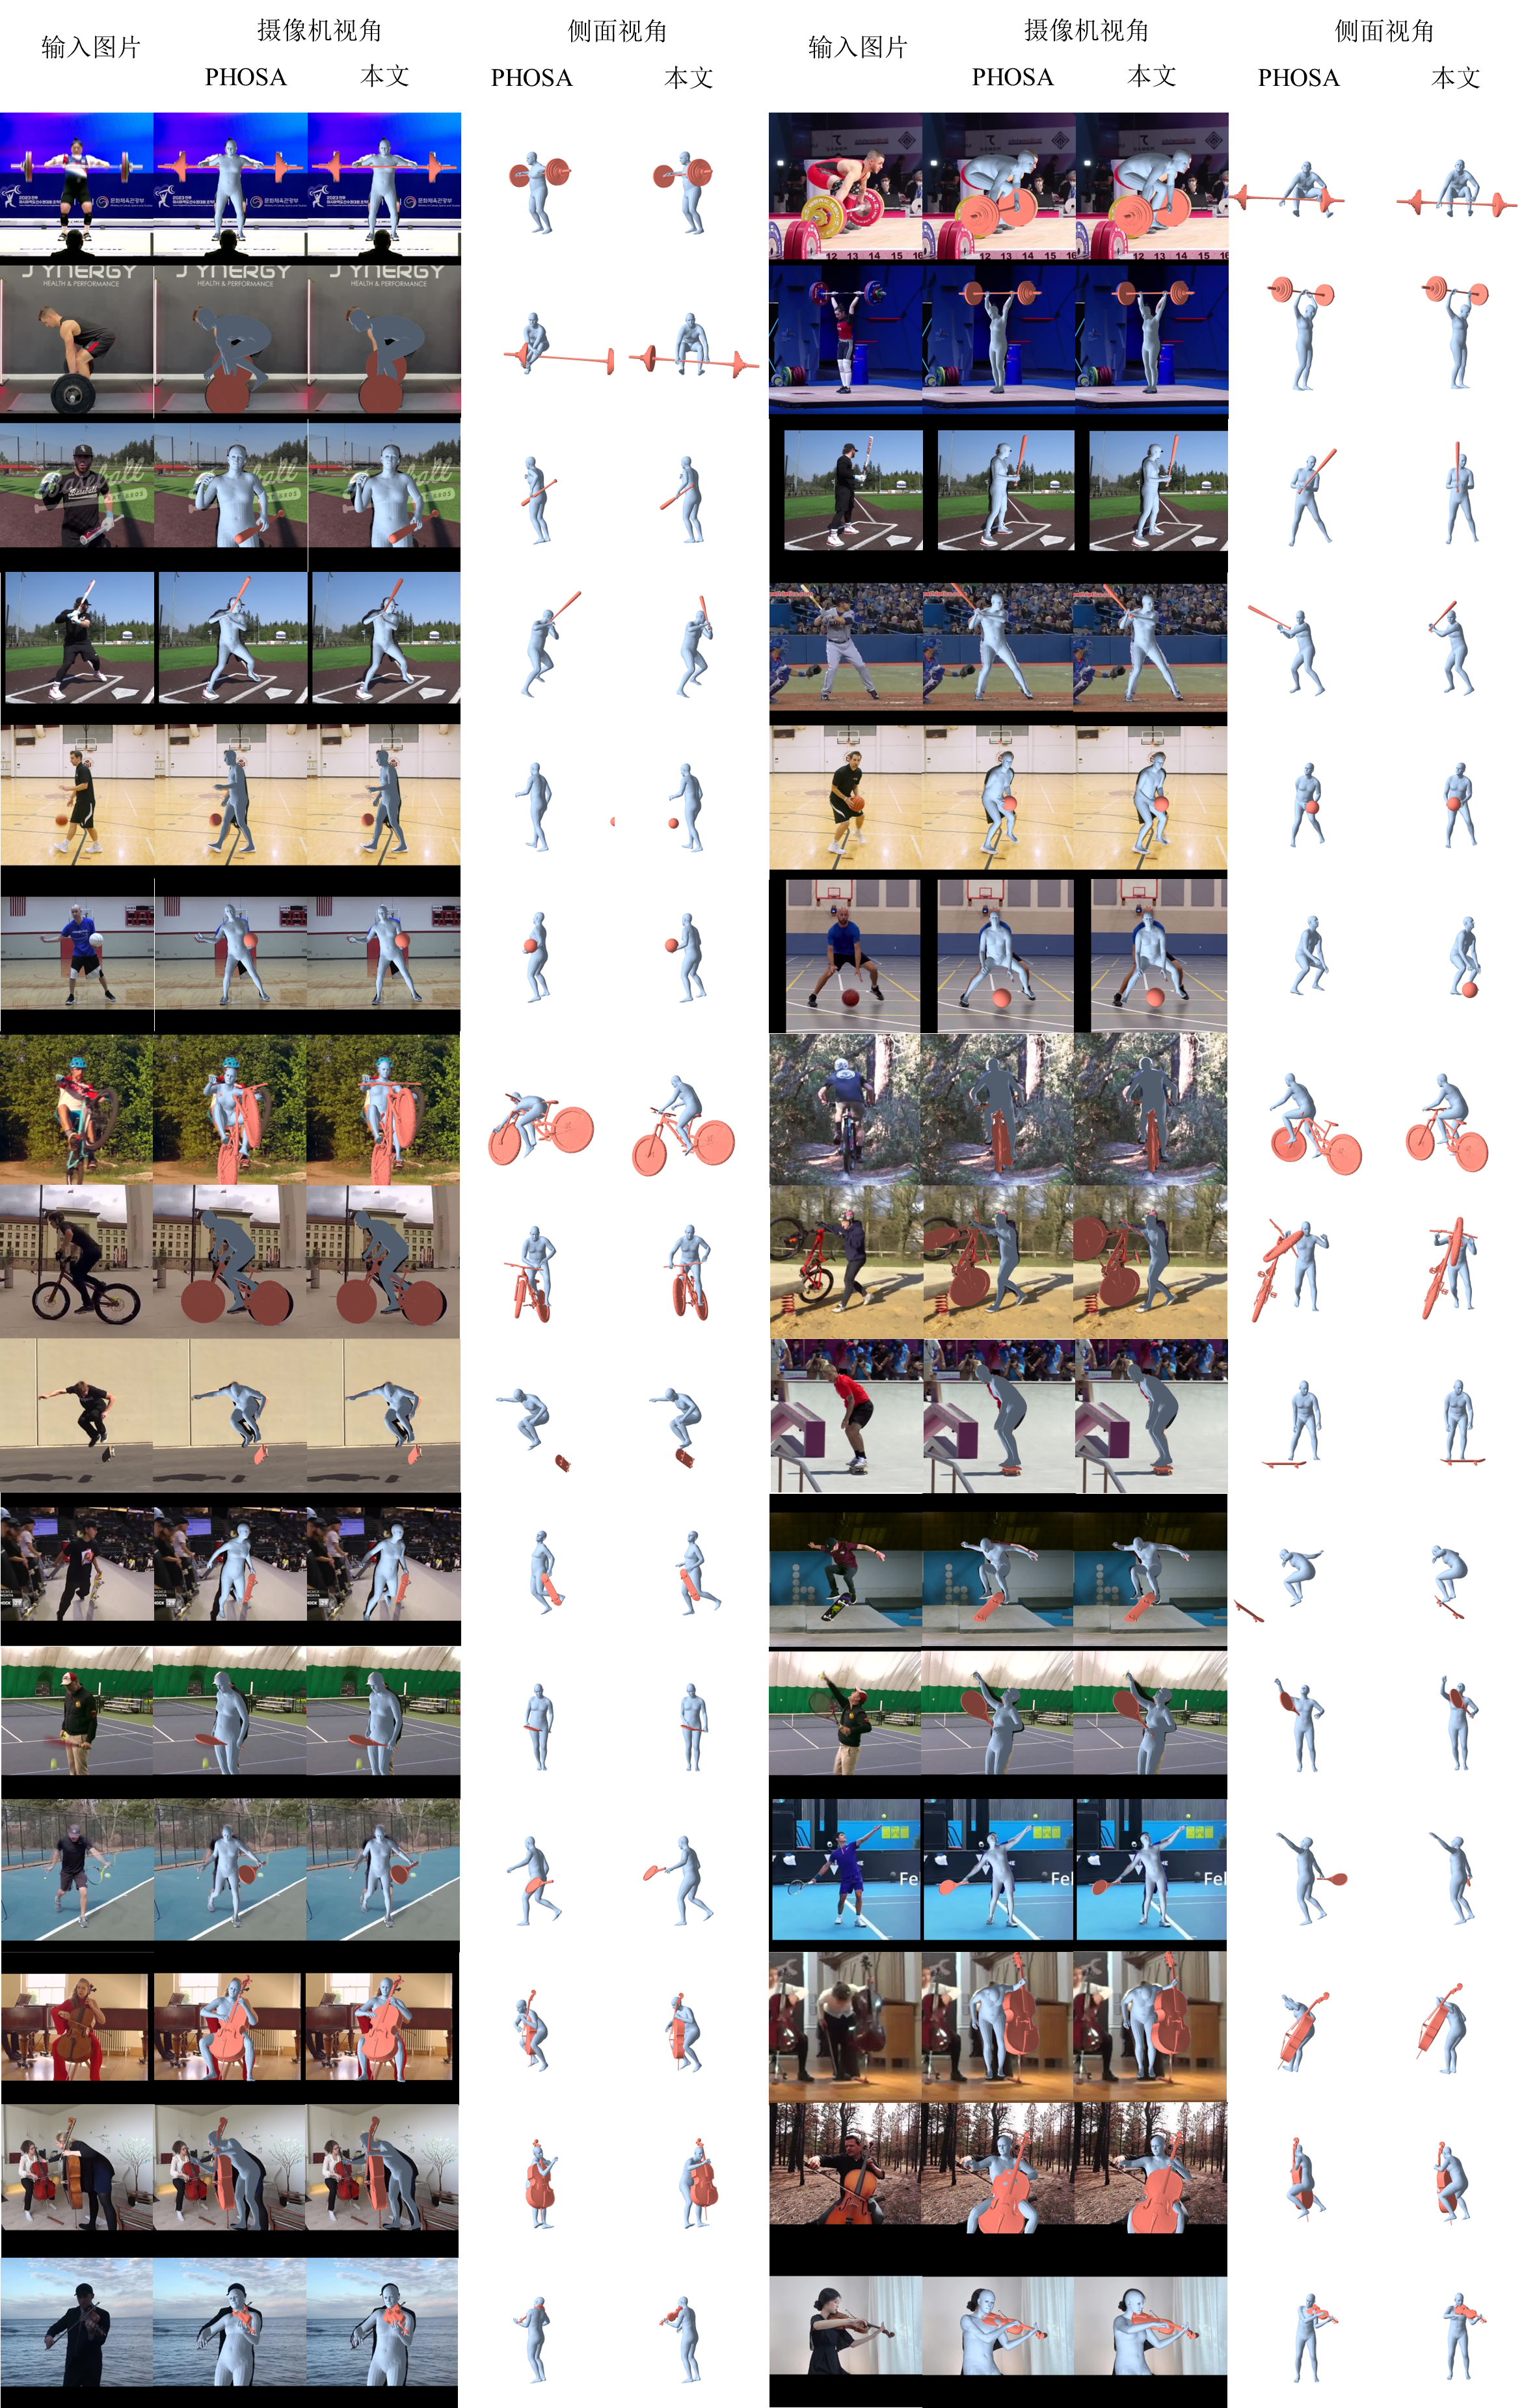
\includegraphics{Img/comparison_2d}
	\bicaption{本章所提出的方法和PHOSA在WildHOI数据集上的定性对比。}{Quantization comparison between our method and PHOSA on WildHOI dataset.}
	\label{fig:comparison-with-phosa}
\end{figure}

% \begin{figure}[!htbp]
% 	\centering
% 	\includegraphics[width=\linewidth]{Img/qualitative_results_sup_2}
% 	\bicaption{本章所提出的方法和PHOSA在WildHOI数据集上的定性对比。}{Quantization comparison between our method and PHOSA on WildHOI dataset.}
% 	\label{fig:comparison-with-phosa2}
% \end{figure}

\begin{figure}[!htbp]
	\centering
	\includegraphics[width=\linewidth]{Img/qualitative_results_sup_3}
	\bicaption{本章所提出的方法和PHOSA在WildHOI数据集上的定性对比。}{Quantization comparison between our method and PHOSA on WildHOI dataset.}
	\label{fig:comparison-with-phosa3}
\end{figure}

\begin{figure}[!htbp]
	\centering
	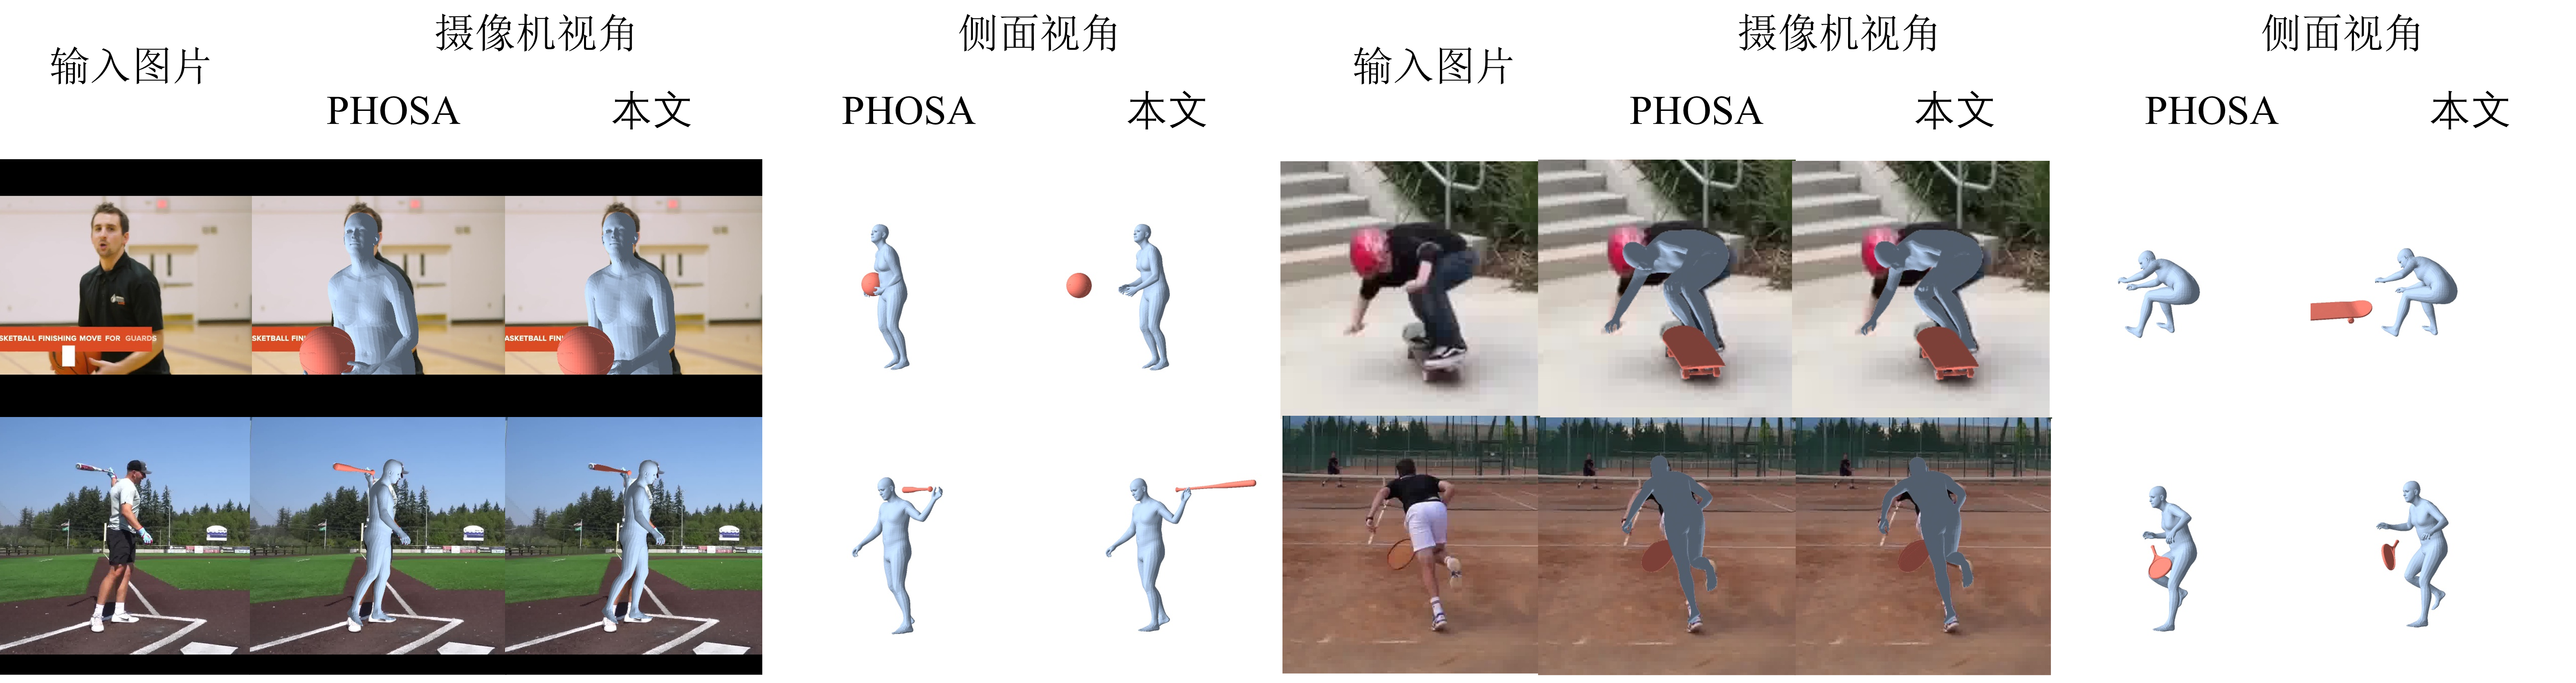
\includegraphics[width=0.9\linewidth]{Img/failures_2}
	\bicaption{在WildHOI-test数据集上的失败样例。}{Failures on WildHOI-test dataset.}
	\label{fig:failures}
\end{figure}

\paragraph{接触面损失和多视角二维关键点损失的有效性}
在表\ref{tab:ablation_contact_loss}中展示了对不同优化损失进行消融实验的结果。从实验结果可以看出,引入先验损失和接触面损失会带来最佳性能,除了在SMPL的倒角距离外,它在所有指标中达到最低的重建误差,这表明先验损失和接触面损失在优化过程发挥着重要作用。通过比较第三行和最后一行,可以看到去掉先验损失会导致重建准确度显著下降,这表明先验损失对重建精度有着更重要的影响。

\begin{table}[!htbp]
	\bicaption{\centering{不同损失对重建结果的影响。}}{\centering{The effectiveness of different losses on the reconstruction accuracy.}}
	\label{tab:ablation_contact_loss}
	\centering
	\footnotesize
	\setlength{\tabcolsep}{4pt}
	\renewcommand{\arraystretch}{1.2}
	\begin{tabular}{cccccc}
		\toprule
		$\mathcal{L}_{\text{prior}}$ & $\mathcal{L}_{\text{contact}}$ & SMPL (cm) $\downarrow$ & Obj. (cm) $\downarrow$ & Rot.($^\circ$) $\downarrow$ & Transl.(cm) $\downarrow$ \\
		\hline
		\XSolidBrush & \XSolidBrush & \textbf{3.57} & 1259.57 & 7.12 & 658.16 \\
		\XSolidBrush & \Checkmark & 3.71 & 363.40 & 6.47 & 195.62 \\
		\Checkmark & \XSolidBrush & 4.36 & 19.37 & 10.26 & 14.26 \\
		\Checkmark & \Checkmark & 4.43 & \textbf{17.48} & \textbf{10.12} & \textbf{13.13} \\
		\bottomrule
		\multicolumn{5}{l}{注:加粗字体为最优结果。}
	\end{tabular}
\end{table}

\paragraph{训练集规模对重建结果的影响} 在表\ref{tab:size_of_training_set}中比较使用不同规模的数据集训练的模型对重建结果的影响,越大的训练集可以带来更准确的重建结果,但微弱的指标提升表明训练集大小并不是影响模型重建精度的主要因素。

\begin{table}[!htbp]
	\bicaption{\centering{训练集大小对重建结果的影响。}}{\centering{The effectiveness of the size of training set on the reconstruction accuracy.}}
	\label{tab:size_of_training_set}
	\centering
	\footnotesize
	\setlength{\tabcolsep}{4pt}
	\renewcommand{\arraystretch}{1.2}
	\begin{tabular}{cccccc}
		\toprule
		训练集 & 测试集 & SMPL (cm) $\downarrow$ & Obj. (cm) $\downarrow$ & Rot.($^\circ$) $\downarrow$ & Transl.(cm) $\downarrow$ \\
		\hline
		50\% & 0\% & 4.48 & 18.53 & 10.41 & 13.76 \\
		75\% & 0\% & 4.31 & 18.15 & 10.35 & 13.33 \\
		100\% & 0\% & 4.43 & 17.48 & 10.12 & 13.13 \\
		100\% & 100\% & 4.34 & 18.07 & 10.40 & 13.44 \\
		\bottomrule
	\end{tabular}
\end{table}

\section{本章小结}
在本章中,探讨了如何从自然场景的二维图像中学习人和物体之间的空间关系的强先验。通过大量实验,展示了即使在不使用任何三维标注或者人体和物体之间三维空间关系的常识的前提下,本章所提出的方法可以在室内实验室场景下构建BEHAVE数据集和室外场景的WildHOI数据集上取得很好的结果。然而,本章所提出的工作仍然存在一些局限性。首先,该方法假设物体的形状是已知的,只聚焦于学习人体和物体的三维空间关系先验。这在物体形状变化很大的真实场景中并不太实用。此外,该方法严重依赖于大量的二维标注数据,而大规模的二维图片数据集并不是容易获得或者这种监督方式并不适用于所有任务。最后,该方法学习的是实例级别的先验而不是类别级先验,这可能对影响到对未见或稀有物体的泛化能力。

未来的研究方向可以包括以下几个方面的改进:
\begin{enumerate}
	\item 考虑物体形状的不确定性:可以引入形状建模和几何推理的方法,以适应不同形状的物体,并进一步提高模型的泛化能力。
	\item 减少对大量二维标注数据的依赖:可以探索使用弱监督或无监督学习的方法,减少对大量标注数据的需求,提高模型的数据利用效率。
	\item 学习类别级的空间关系先验:可以尝试引入类别信息,学习不同物体类别之间的空间关系先验,提高模型对不同类别的泛化能力。
\end{enumerate}

通过进一步探索和改进,可以使该方法在更广泛的应用场景中取得更好的效果,并为实际场景中的人体与物体关系推理提供更有效的解决方案。